\documentclass[a4paper,14pt]{extarticle}

\usepackage[utf8]{inputenc}
\usepackage[T2A]{fontenc}
\usepackage[english, russian]{babel}

\usepackage[mode=buildnew]{standalone}
\usepackage{setspace}


% Различные пакеты
\usepackage{
	amssymb, amsfonts, amsmath, amsthm, physics,
	cancel, indentfirst,makecell,multirow, 
	graphicx, tikz, mathtools, float, setspace,caption,subcaption
} 

\usepackage{mathtools}

% Эта опция включает нумерацию только у тех формул,
% на которые есть ссылка в документе
\mathtoolsset{showonlyrefs=true} 

 % Цвета для гиперссылок
\definecolor{linkcolor}{HTML}{000000} % цвет ссылок
\definecolor{urlcolor}{HTML}{799B03} % цвет гиперссылок
 
\usepackage{xcolor}
\usepackage[
    unicode, 
    colorlinks, 
    urlcolor=urlcolor, 
    linkcolor=linkcolor,
    citecolor=linkcolor
]{hyperref}

% Увеличенный межстрочный интервал, французские пробелы
\linespread{1.2} 
\frenchspacing 

%%%%%%%%%%%%%%%%%%%%%%%%%%%%%%
%  Пользовательские команды  %
%%%%%%%%%%%%%%%%%%%%%%%%%%%%%%


\makeatletter
    \newcommand{\fftStar}[1]{\mathfrak{F}^*\qty[#1]}
    \newcommand{\fftNoStar}[1]{\mathfrak{F}\qty[#1]}
    \newcommand{\fft}{
                 \@ifstar
                 \fftStar%
                 \fftNoStar%
    }
\makeatother

\makeatletter
    \newcommand{\ifftNoStar}[1]{\mathfrak{F}^{-1}\qty[#1]}
    \newcommand{\ifftStar}[1]{\qty(\mathfrak{F}^{-1}\qty[#1])^*}
    \newcommand{\ifft}{
                 \@ifstar
                 \ifftStar%
                 \ifftNoStar%
    }
\makeatother

\newcommand{\mean}[1]{\langle#1\rangle}
\newcommand\ct[1]{\text{\rmfamily\upshape #1}}
\newcommand*{\const}{\ct{const}}
\renewcommand{\phi}{\varphi}
\renewcommand{\epsilon}{\varepsilon}
%\renewcommand{\sigma}{\varsigma}


\captionsetup{subrefformat=parens}

\usepackage{array}
\usepackage{pstool}


% Диагональная ячейка в таблице ( типа |a/b|)
\newcolumntype{x}[1]{>{\centering\arraybackslash}p{#1}}
\newcommand\diag[4]{%
  \multicolumn{1}{p{#2}|}{\hskip-\tabcolsep
  $\vcenter{\begin{tikzpicture}[baseline=0,anchor=south west,inner sep=#1]
      \path[use as bounding box] (0,0) rectangle (#2+2\tabcolsep,\baselineskip);
      \node[minimum width={#2+2\tabcolsep},minimum height=\baselineskip+\extrarowheight] (box) {};
      \draw (box.north west) -- (box.south east);
      \draw (box.south west) -- (box.north west);
      \node[anchor=south west] at (box.south west) {\footnotesize#3};
      \node[anchor=north east] at (box.north east) {\footnotesize#4};
 \end{tikzpicture}}$\hskip-\tabcolsep}}

%%%%%%%%%%%%%%%%%%%%%%%%%%%%%
%  Геометрия и колонтитулы  %
%%%%%%%%%%%%%%%%%%%%%%%%%%%%%


\usepackage{geometry}
\geometry       
    {
        left            =   2cm,
        right           =   2cm,
        top             =   2.5cm,
        bottom          =   2.5cm,
        bindingoffset   =   0cm
    }

% Настройка содержания, точки после нумераций
\usepackage{tocloft}
\addto\captionsrussian{\renewcommand{\contentsname}{Оглавление}}
\renewcommand{\cftsecleader}{
	\cftdotfill{\cftdotsep}}
% \renewcommand{\thesection}{
	% \arabic{section}.}
% \renewcommand{\thesubsection}{
	% \arabic{section}.\arabic{subsection}.}
% \renewcommand{\thesubsubsection}{
	% \arabic{section}.\arabic{subsection}.\arabic{subsubsection}.}     
\usepackage[explicit]{titlesec}

% Колонтитулы
%\usepackage{fancyhdr} 
	%\pagestyle{plain} 
	%\fancyhead{} 
	%\fancyhead[R]{} 
	%\fancyhead[L]{} 
	%\fancyfoot{} 
	%\fancyfoot[C]{\thepage} 

\NewDocumentCommand{\codeword}{v}{%
\texttt{\textcolor{gray}{#1}}%
}
\usepackage{listings,multicol}
\usepackage{courier}
\definecolor{mygreen}{rgb}{0,0.6,0}
\definecolor{mygray}{rgb}{0.5,0.5,0.5}
\definecolor{mymauve}{rgb}{0.58,0,0.82}
\newcommand{\python}[1]{\lstinline[basicstyle=\normalsize\ttfamily]{#1}}

\lstset{ 
  backgroundcolor=\color{white},   % choose the background color; you must add \usepackage{color} or \usepackage{xcolor}; should come as last argument
  basicstyle=\footnotesize\ttfamily,        % the size of the fonts that are used for the code
  breakatwhitespace=false,         % sets if automatic breaks should only happen at whitespace
  breaklines=true,                 % sets automatic line breaking
  captionpos=b,                    % sets the caption-position to bottom
  commentstyle=\color{mygreen},    % comment style
  deletekeywords={...},            % if you want to delete keywords from the given language
  escapeinside={\%*}{*)},          % if you want to add LaTeX within your code
  extendedchars=true,              % lets you use non-ASCII characters; for 8-bits encodings only, does not work with UTF-8
  firstnumber=1,                % start line enumeration with line 1000
  frame=single,	                   % adds a frame around the code
  keepspaces=true,                 % keeps spaces in text, useful for keeping indentation of code (possibly needs columns=flexible)
  keywordstyle=\color{blue},       % keyword style
  language=Python,                 % the language of the code
  morekeywords={*,...},            % if you want to add more keywords to the set
  numbers=left,                    % where to put the line-numbers; possible values are (none, left, right)
  numbersep=15pt,                   % how far the line-numbers are from the code
  numberstyle=\tiny\color{mygray}, % the style that is used for the line-numbers
  rulecolor=\color{black},         % if not set, the frame-color may be changed on line-breaks within not-black text (e.g. comments (green here))
  showspaces=false,                % show spaces everywhere adding particular underscores; it overrides 'showstringspaces'
  showstringspaces=false,          % underline spaces within strings only
  showtabs=false,                  % show tabs within strings adding particular underscores
  stepnumber=1,                    % the step between two line-numbers. If it's 1, each line will be numbered
  stringstyle=\color{mymauve},     % string literal style
  tabsize=2,	                   % sets default tabsize to 2 spaces
  %title=\lstname,                   % show the filename of files included with \lstinputlisting; also try caption instead of title
  frame=none,
  %multicols=1,
  columns=fullflexible,
  extendedchars=\true,
  escapechar=!,
}




\title{Компьютерные технологии}
\author{Горев С.}



\begin{document}
\maketitle

\textbf{Задание 8} Рассчитайте эффективную траекторию ракеты, предназначенной для наименее
затратного по топливу запуска с Земли искусственного спутника Марса. Постройте зависимости
скорости и координаты ракеты от времени, а также оцените точность интегрирования в
зависимости от схемы интегрирования и величины шага интегрирования

\section{Подход к решению задачи}
Оптимальной по топливу траекторией перехода с одной орбиты на другую является
Гомановская траектория - в ходе нее ракета выполняет два импульса - начальный $\Delta V_1$,
для достижения конечной орбиты, и конечный $\Delta V_2$, для выхода на конечную орбиту.
В данном решении будет использоваться Гомановская траектория полета - т.е. всего будет два импульса приращения скорости.

Теоретические значения приращения скорости
\begin{equation}
	\Delta V_1 = V_E \left(\frac{V_E}{V_p}-1\right), \quad \Delta V_2 = V_M \left(1- \frac{V_M}{V_p}\right),
\end{equation}
где $V_E, V_M$ - орбитальные скорости Земли и Марса, $V_p = \sqrt{\frac{V_E^2 + V_M^2}{2}}$. Однако, данные значения справедливы
только когда не учитывается гравитационное притяжение тел (Земли, Марса), поэтому при учете этих сил
траектория будет искажена. В данной работе значение первого импульса будет находится путем оптимизации, условием которой будет
достижение геостационарной орбиты (ГСО) Марса, при минимальной радиальной скорости ракеты при сближении.

\section{Описание системы тел}
В нашем случае система состоит из Солнца, Земли, Марса и ракеты. Орбиты планет будет считать круговыми, с фиксированными
радиусами и орбитальными скоростями. Солнце неподвижно и расположено в начале координат.

Ракета будет запускаться с ГСО Земли, при этом будет расположена от Солнца дальше, чем Земля. Таким образом, начальные
параметры ракеты можно записать как 
\begin{equation}
		x(0) = R_E + GSO_E, y(0) = 0, V_x(0)=0, V_y(0) = V_E + V_{GSO, E} + \Delta V_1
\end{equation}
, где $R_E=1.5 \cdot 10^{11}$ м - радиус орбиты Земли, $GSO_E = 6.371 \cdot 10^6 + 35.786 \cdot 10^6 = 42.157 \cdot 10^6$ м -
величина радиуса ГСО Земли, при отсчете от центра Земли, $V_{GSO, E} = 3065$ м/с - скорость на ГСО Земли.

Важным параметром является момент, в который ракета производит запуск с ГСО Земли по отношению к положению Марса.
В данной работе оптимальное положение Марса будет находится путем оптимизации тем же методом, что и нахождение оптимального
начального импульса.

Таким образом, в задаче будут следующие ключевые этапы:
\begin{enumerate}
	\item Ракета начинает движение с ГСО Земли. Движение ракеты описывается всемирным законом тяготения.
	\item Определяется оптимальный начальный импульс, путем минимизации некоторой функции $M=M(\Delta V_1, \theta_M(0))$, 
	где $\theta_M(0)$ - начальный угол положения Марса в полярных координатах.
	\item Найдя оптимальные значения $\Delta V_1, \theta_M(0)$, рассчитывается полет ракеты до Марса, до момента максимального
	сближения.
	\item Дальше ракете придается дополнительный импульс $\Delta V_2$, после которого ракета выходит на орбиту Марса.
\end{enumerate}


\section{Описание движения ракеты в системе}
Для моделирования влияния нескольких тел на движение ракеты, воспользуемся вторым законом Ньютона и законом
всемирного тяготения:
\begin{equation}
	\vec{F} = m\vec{a} = \vec{F_g} = G m \sum_{i=0}^{N-1}\frac{m_i}{R_i^2}\vec{e_i},
\end{equation}
где $i$ - индекс, $m$ - масса ракеты, $m_i$ - масса $i$-ого тела, $R_i$ - расстояние между
ракетой и $i$-м телом, $\vec{e_i}$ - единичный вектор, направленный от ракеты к телу с индексом $i$.
Влияние ракеты на движение планет и Солнца не учитывается.

Учтем, что $\vec{r''}=\vec{a}, \vec{r'} = \vec{v}$, тогда
\begin{equation}
	\vec{v'} = G \sum_{i=0}^{N-1}m_i\frac{\vec{r_i}-\vec{r}}{R_i^3}, \quad
	\vec{r'} = \vec{v}
\end{equation}
где $\vec{r_i}$ - радиус вектор положения тела с индексом $i$.
Решением полученной системы уравнений будет траектория полета ракеты $\vec{r}(t), \vec{v}(t)$.
Именно эта системы и будет моделироваться в программе.

\section{Определение оптимальных параметров}
Ранее была введена функция $M=M(\Delta V_1, \theta_M(0))$, минимизацией значения которой будут найдены оптимальные 
параметры $\Delta V_1, \theta_M(0)$. Опишем критерии, по которым будет определяться нахождение оптимальных параметров.
\begin{enumerate}
	\item Критерий достижения ГСО Марса. Минимальное расстояние до Марса должно быть меньше или равно величине
	ГСО Марса (считая от центра координаты Марса)
	\item Минимальная радиальная скорость. Радиальная скорость ракеты при минимальном расстоянии до Марса должна быть минимальной, в идеале 0.
	\item Оптимальная траектория полета. Максимальное значение радиуса орбиты ракеты должно быть близко к значению орбиты Марса.
\end{enumerate}
Исходя из поставленных критериев была составлена функция, возвращаемое значение которой является
\begin{equation}
	M=M(\Delta V_1, \theta_M(0)) = \abs{d2M_{min}} + V_{r min}^2 + \abs{d2MO},
\end{equation}
где $d2M_{min}$ - расстояние до ГСО Марса при максимальном сближении, $V_{r min}$ - радиальная скорость при максимальном сближении,
$d2MO$ - разность между максимальным радиусом орбиты ракеты и орбитой Марса.
Минимизируя данную величину, будут найдены оптимальные параметры $\Delta V_1, \theta_M(0)$.

\section{Результаты моделирования}
Моделирование системы производится на языке Python.
Используется библиотека SciPy и метод \text{integrate.solve\_ivp}.
В методе \text{integrate.solve\_ivp} использует алгоритм Рунге-Кутты 5-го порядка ('Radau'). Шаг интегрирования выбирается так,
чтобы ошибка не превышала наперед заданного значения относительной $\varepsilon_r \leq 10^{-3}$ и абсолютной
ошибок $\varepsilon_a \leq 10^{-6}$ интегрирования.

Исходный код приведен в листинге \ref{lst:task9}.

Результаты моделирования приведены на рисунках \ref{fig:trj}, \ref{fig:crds}, \ref{fig:vel}.

Изначальные значения $\Delta V_1=2400 m/s, \theta_M(0)=0.91 rads$. Начальные координаты и скорости ракеты
\begin{equation}
	x(0) = 1.5 \cdot 10^{11} + 42.157 \cdot 10^6, y(0) = 0, V_x(0)=0, V_y(0) = 29783 + 3065 + \Delta V_1
\end{equation}

Оптимальные значения $\Delta V_1, \theta_M(0)$, найденные в ходе оптимизации
\begin{equation}
	\Delta V_1^{opt} = 2327.05 m/s \quad \theta_M(0)^{opt} = 0.925 rads,
\end{equation}
для сравнения, теоретической значение $\Delta V_1=2943.45$ м/с, однако из-за влияния гравитации Земли
оптимальное значение отличается от теоретического.

Момент достижения Марса отмечен на графиках вертикальной линией, и составляет $t_{ETA} = 261.13$ дней с момента запуска.
В момент достижения Марса сближение с центром Марса составляет $10475$ км, при величине ГСО Марса $20389.5$ км. Радиальная скорость
при максимальном сближении составляет $-258$ м/с.

После достижения Марса, ракете придается второй импульс $\Delta V_2 = 2647.9$ м/с, что является теоретическим значением.
После этого, ракета выходит на орбиту Марса, что можно пронаблюдать на графике скорости на рис. \ref{fig:vel} - после момента достижения Марса,
скорость начинает сильно осциллировать, что характерно при выходе на орбиту планеты. Также приведен график координаты в увеличенном мастшатбу на рис. 
\ref{fig:orb}, на котором наблюдается осцилляция вокруг координаты Марса.

\begin{figure}
	\center
	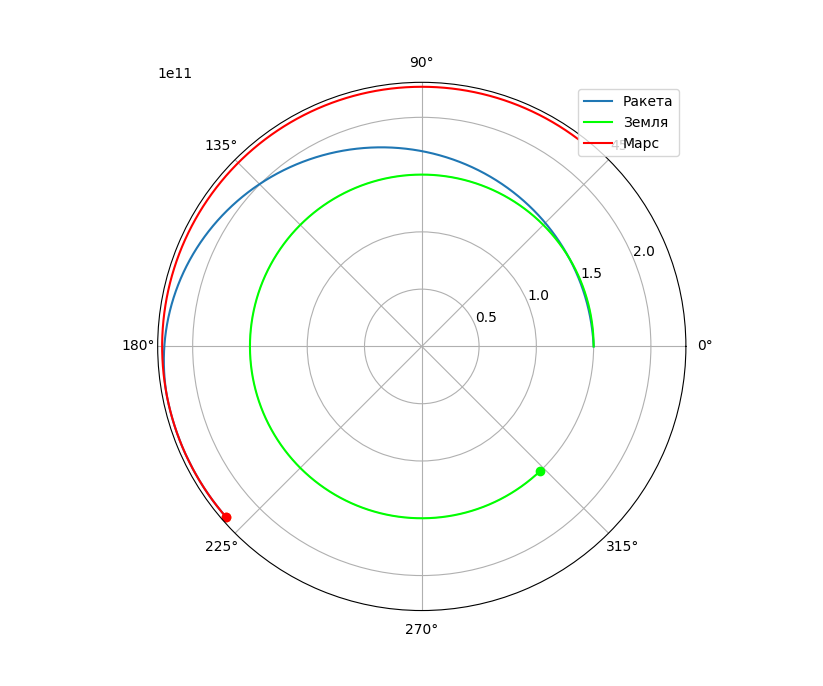
\includegraphics[width=.8\linewidth]{imgs_9/trj.png}
	\caption{Траектории движений}
	\label{fig:trj}
\end{figure}

\begin{figure}
	\center
	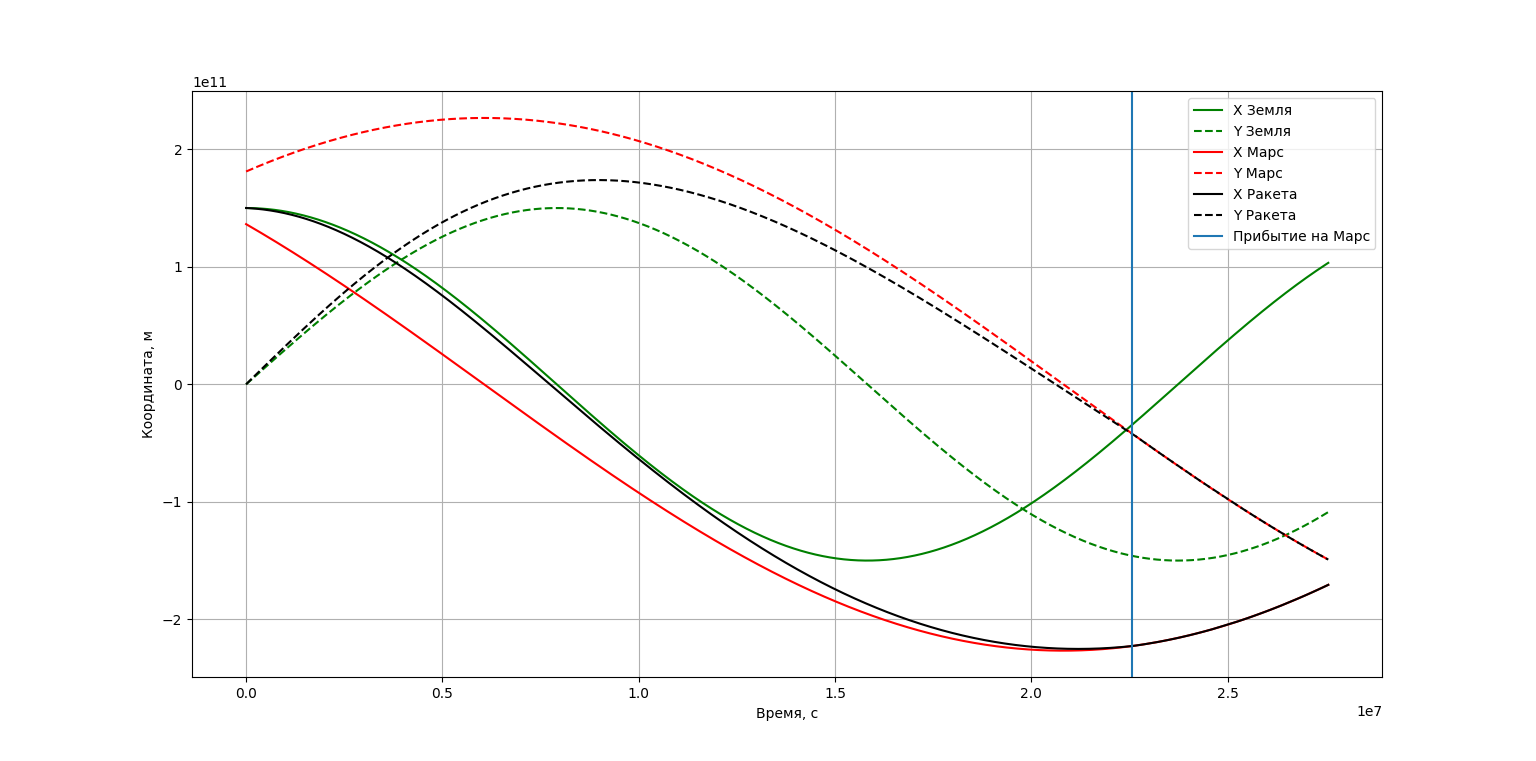
\includegraphics[width=.99\linewidth]{imgs_9/crds.png}
	\caption{Координаты от времени}
	\label{fig:crds}
\end{figure}

\begin{figure}
	\center
	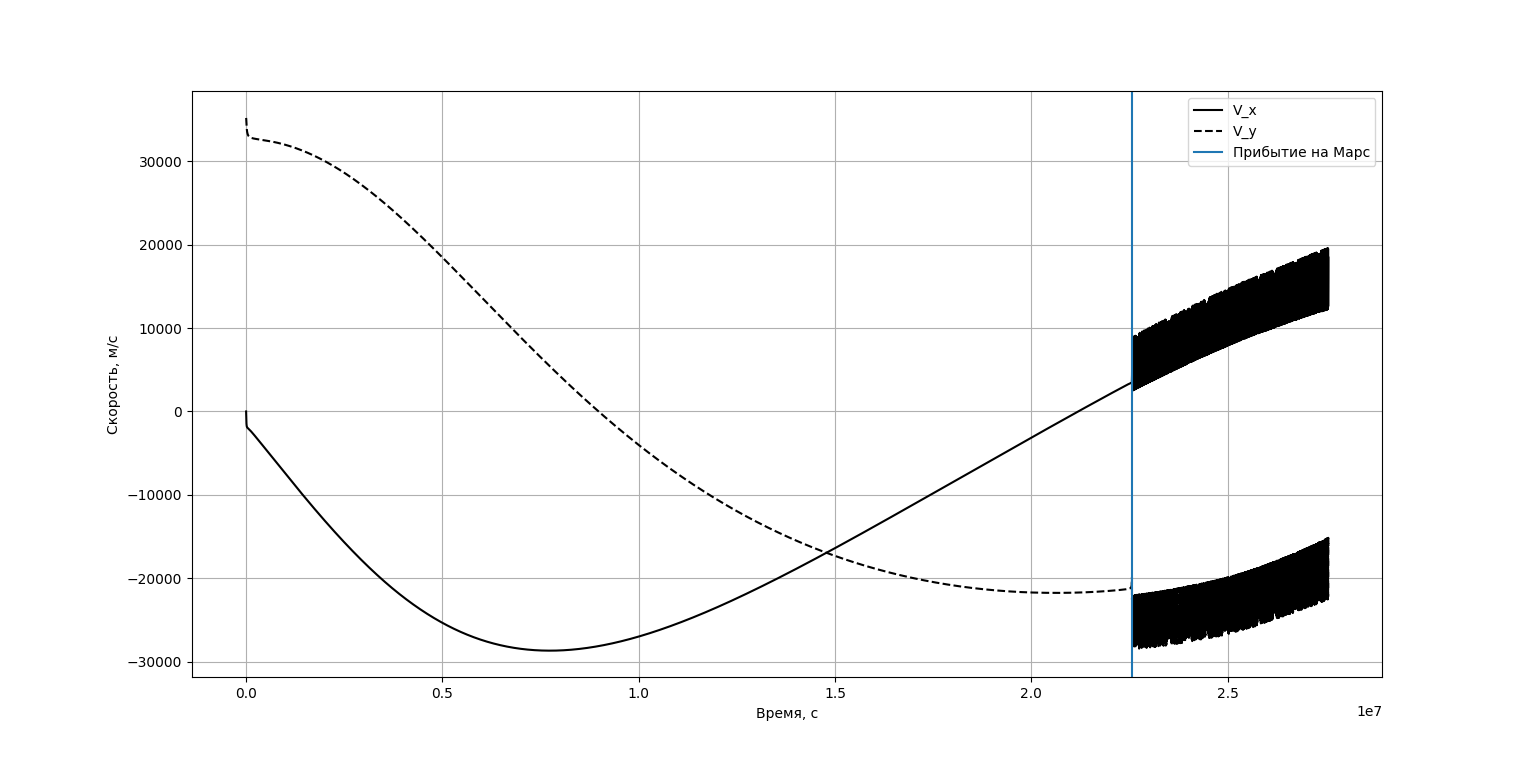
\includegraphics[width=.99\linewidth]{imgs_9/vel.png}
	\caption{Скорость ракеты от времени}
	\label{fig:vel}
\end{figure}

\begin{figure}
	\center
	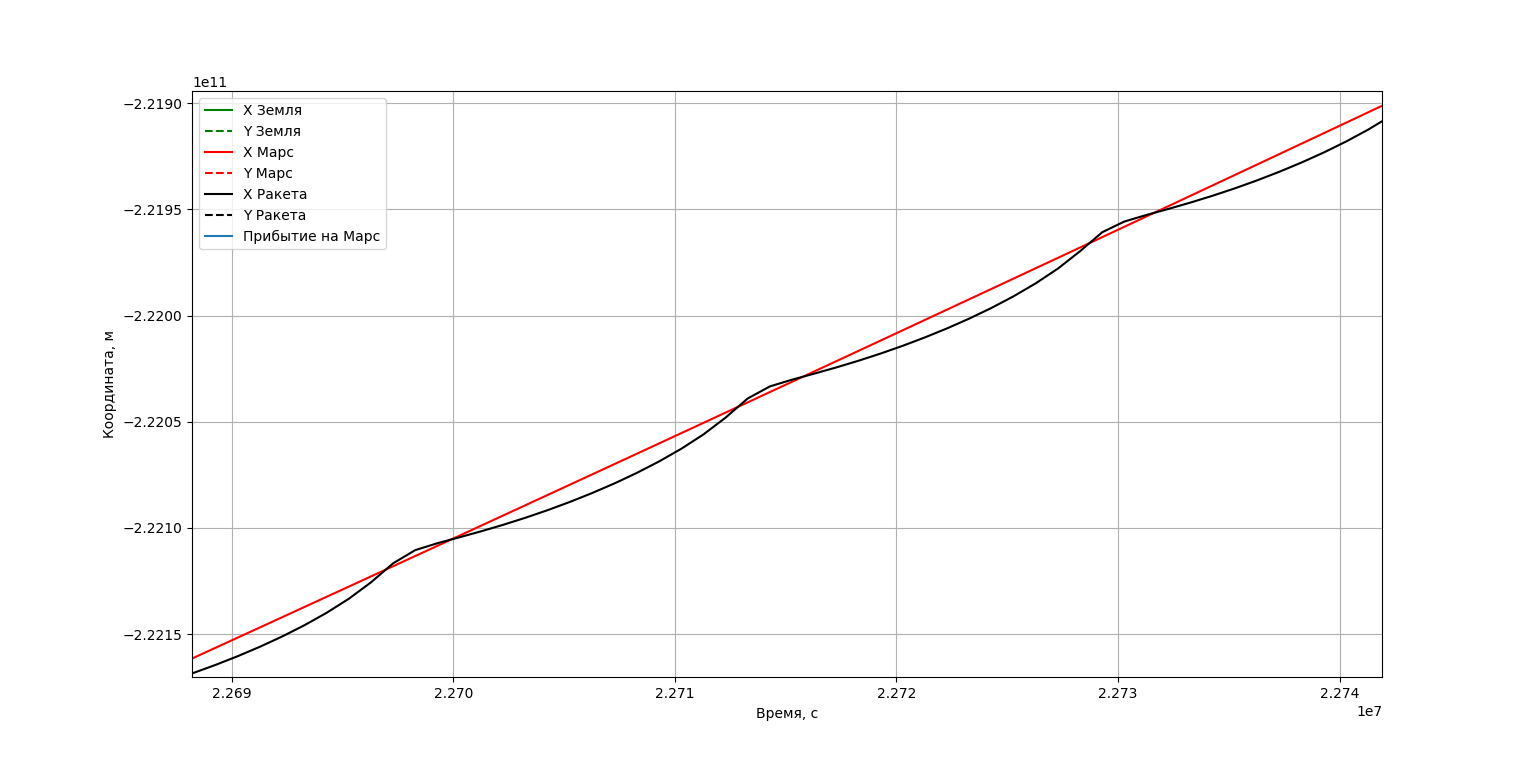
\includegraphics[width=.99\linewidth]{imgs_9/orb.png}
	\caption{Выход ракеты на орбиту Марса - координата ракеты осциллирует вокруг координаты Марса}
	\label{fig:orb}
\end{figure}

\newpage
\section{Исходный код}
\lstinputlisting[label={lst:task9}, caption={Исходный код задания}]{task_9.py}


\end{document}